\newpage
\thispagestyle{fancy}

\begin{center}
	\huge\textbf{GEI 752 : Travail pratique}
	\bigbreak
	\LARGE\textbf{Traitement de signaux EEG et applications dans une interface cerveau-ordinateur}
	\bigbreak
\end{center}

\normalsize

On vous propose à travers ce travail pratique de vous familiariser avec les aspects théoriques et techniques d'une interface cerveau-ordinateur et d'utiliser vos connaissances en traitement du signal afin de participer à la conception de la chaine de traitement des données électroencéphalographiques (EEG).

\newpage
\section*{Interface cerveau-ordinateur}

Une interface Cerveau-Ordinateur ou BCI (Brain Computer Interface) est une interface permettant de réaliser une communication allant du cerveau vers un système numérique (ordinateur par exemple). Pour cela, on s'appuie sur une étude de l'activité neuronale du cerveau grâce à un système électroencéphalographique (EEG) utilisant des électrodes. Celles-ci sont placées à la surface du crâne afin de capter son activité électrique. Un traitement et une analyse des signaux électriques saisis sont réalisés afin de les traduire en informations exploitables par les systèmes numériques. L'expérience que l'on vous propose d'étudier ici s'appuie sur la méthode d'imagerie motrice, qui consiste à imaginer le mouvement de différentes parties du corps. Cela résulte en l'activation du cortex sensorimoteur qui module certains rythmes du cerveau. Ces variations peuvent être détectées par des électrodes EEG. L'interface cerveau-ordinateur en déduit les intentions de l'utilisateur à partir de ces signaux. Dans notre cas, celle-ci doit être capable de déterminer si l'utilisateur pense à un mouvement de sa main droite ou de sa main gauche.

La chaîne de traitement des signaux EEG de l'interface cerveau-ordinateur se compose de 5 étapes (Figure	\ref{fig:interface_travail_ov_5}) : 

\begin{enumerate}
	\item \textbf{L'acquisition des données.} En temps normal, on récupère les données directement issues d'un casque EEG (par exemple le casque EPOC de la société Emotiv). Comme vous ne possédez pas ce genre de casque, on vous fournit un fichier .csv contenant des signaux EEG pré-enregistrés d'une personne pensant aléatoirement à sa main gauche ou droite.
	\smallbreak
	\item \textbf{Filtrage temporel.} Ce filtrage permet d'extraire les rythmes du cerveau qui nous intéressent.
	\smallbreak
	\item \textbf{Filtrage spatial.} On souhait utiliser un filtrage spatial afin d'optimiser nos données. Il vous sera demandé ultérieurement d'implémenter ce filtre sous Matlab. 
	\item \textbf{Filtrage spatial CSP.} Permet de réduire la quantité d'informations à traiter en réalisant une décorrélation et en pondérant certaines des sorties du casque. 
	\smallbreak
	\item \textbf{Analyse spectrale.} Réalise une analyse spectrale via une transformée de Fourier.
	\smallbreak
	\item \textbf{Classification.} Effectue une classification des caractéristiques présentes à son entrée afin de déterminer à quelle main pensait l'utilisateur à un instant donné. 
\end{enumerate}

Le classificateur nécessite d'être préalablement entrainé grâce à d'autres scénarios, qui génèrent alors son fichier de configuration. On vous fournit directement le fichier de configuration ("classifier.cfg"). Veuillez également noter que vous ne possédez pas le scénario d'acquisition permettant de récupérer les données EEG. On vous fournit donc également les données filtrées temporellement dans le fichier ("données\_entrée.csv").

\begin{figure}[h]
	\centering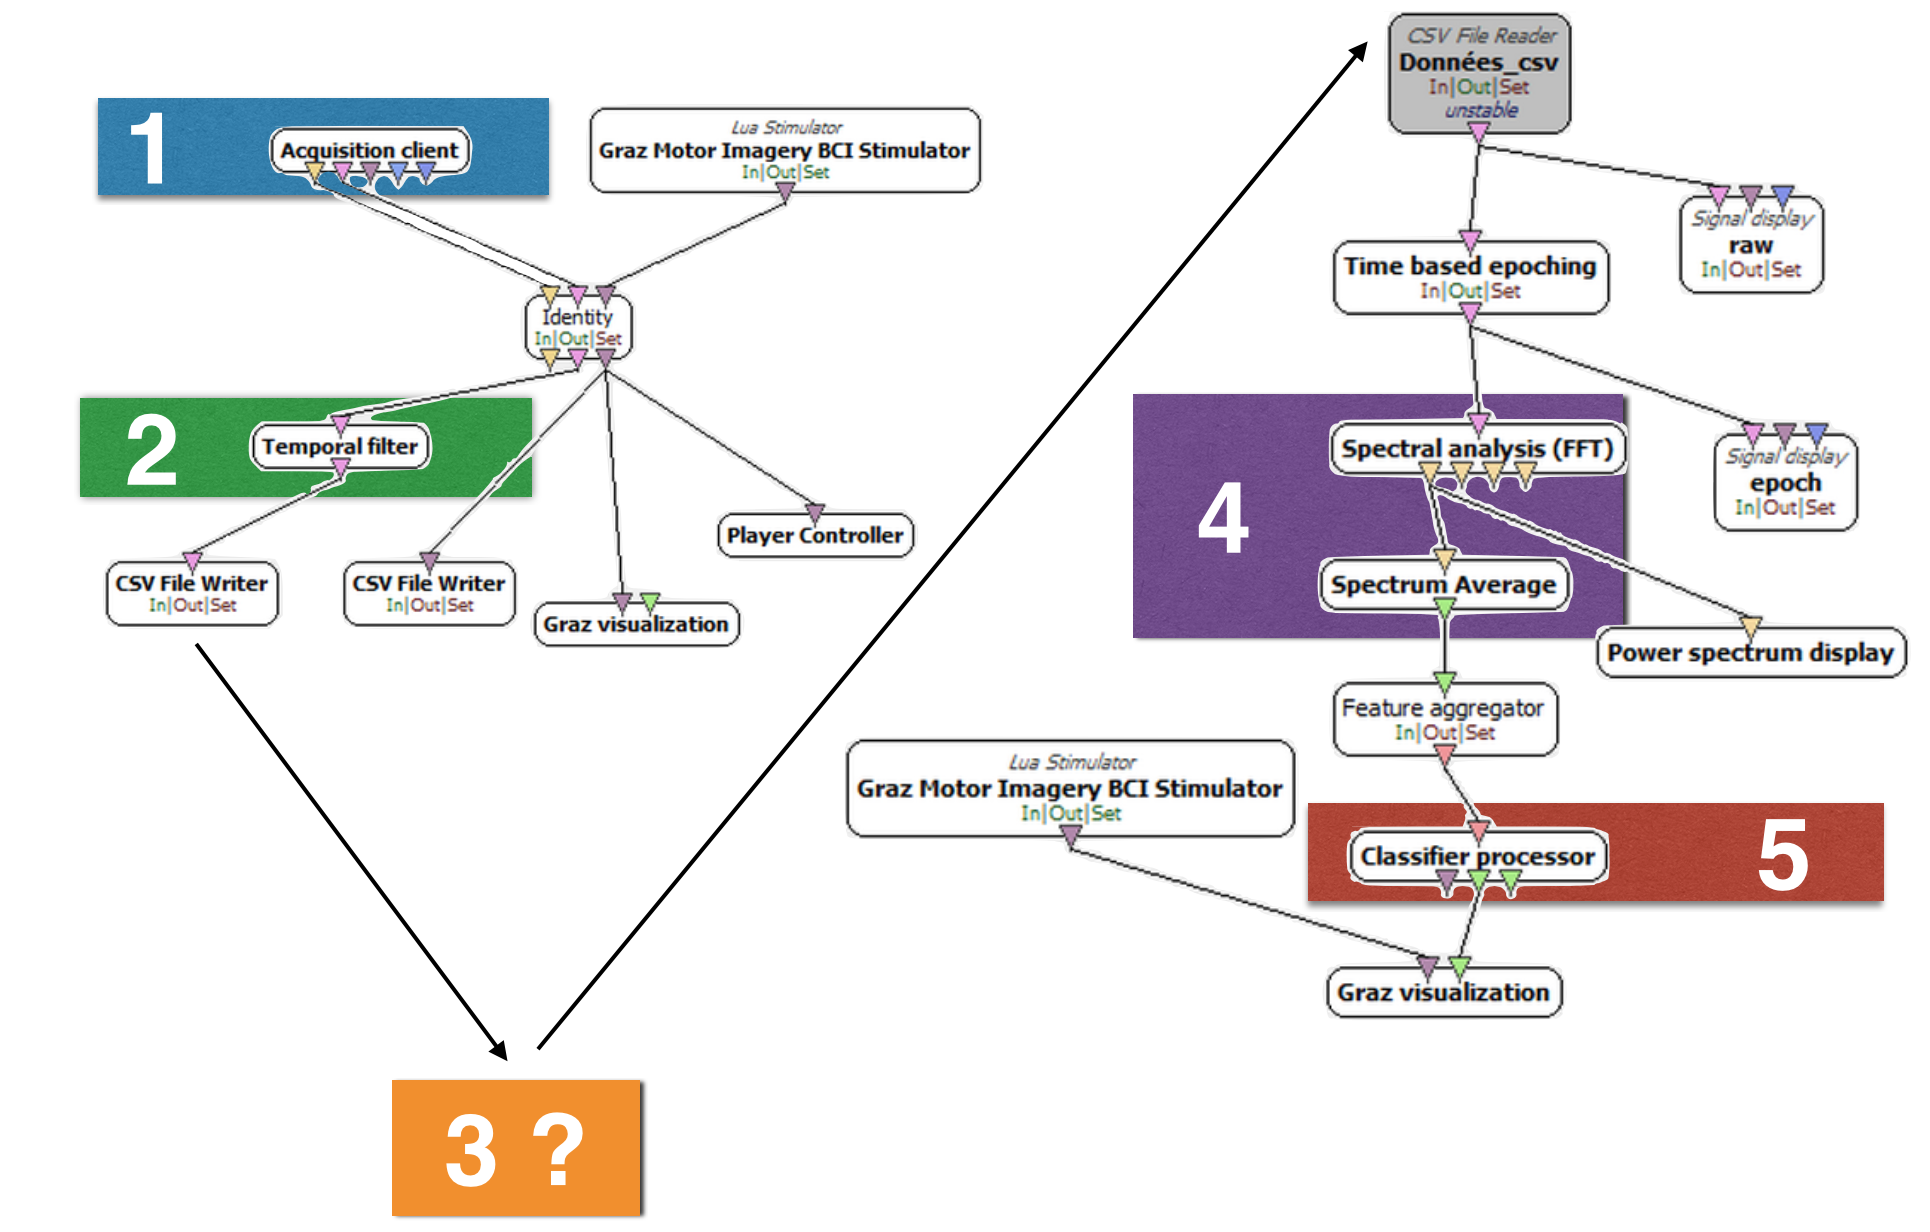
\includegraphics[height=10cm]{images/sujet_signal_color.png}
	\caption{Traitement des signaux EEG sous OpenViBE.}
	\label{fig:interface_travail_ov_5}
\end{figure}

\newpage
\section*{OpenViBE}

\subsection*{Présentation du logiciel}

OpenViBE est une plateforme logicielle dédiée à la conception et à l'utilisation d'interfaces cerveau-ordinateur en temps réel. Celle-ci est éditée par l'Institut National de Recherche en Informatique et en Automatique (INRIA) de Rennes (France). Le logiciel gère à la fois l'acquisition, le traitement et l'analyse des signaux.

Le logiciel fonctionne sous la forme de scénarios, correspondant à un ensemble de blocs fonctionnels. La suite OpenViBE est composée de deux logiciels : 
\begin{itemize}
	\item \textbf{OpenViBE designer}. Il s'agit d'un éditeur de scénario permettant de  créer et modifier les schémas blocs grâce à une interface graphique. Il suffit alors de placer les différents blocs, de les configurer (en cliquant dessus), et de les relier pour former une chaine de traitement.
	\smallbreak
	\item \textbf{OpenViBE acquisition server.} Permet d'acquérir des données EEG brutes à partir de dispositifs EEG. Il est par exemple possible de connecter différents types de casques, dont le casque EPOC.
	\smallbreak
\end{itemize}

\subsection*{Téléchargement et installation d'OpenViBE}

Le logiciel fonctionne sous les systèmes d'exploitations Windows (Windows XP ou ultérieur, la stabilité du logiciel sous Windows 8 n'ayant pas été vérifiée par l'éditeur) et Linux (Ubuntu, Fedora). La liste détaillée des architectures compatibles avec OpenViBE est disponible à l'adresse suivante : http://openvibe.inria.fr/supported-architectures/.
Il est possible de télécharger l'installeur OpenViBE à l'adresse suivante : http://openvibe.inria.fr/downloads/. Une fois celui-ci téléchargé, il suffit de l'ouvrir et de suivre les indications affichées à l'écran.

\subsection*{Présentation de l'interface utilisateur d'OpenViBE Designer}

\subsubsection*{Description de l'interface de contrôle de la simulation}

La partie supérieure de l'interface graphique permet de contrôler la simulation, i.e. le déroulement du scénario. Ainsi, il est possible de lancer un scénario en appuyant sur le bouton "lecture", de le stopper en appuyant sur le bouton "stop" et d'en accélérer le déroulement en appuyant sur le bouton "avance rapide". Il est également possible de lancer plusieurs scénarios en même temps (Figure : \ref{fig:interface_simu_ov_2}). 

\begin{figure}[h]
	\centering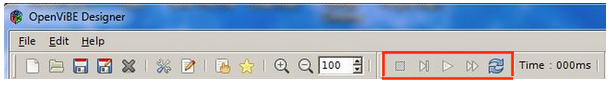
\includegraphics[height=2cm]{images/interface_simu_ov.png}
	\caption{Interface de contrôle de la simulation sous OpenViBE.}
	\label{fig:interface_simu_ov_2}
\end{figure}

\subsubsection*{Description de l'interface du répertoire des blocs fonctionnels}

La partie située à droite de l'interface graphique du designer permet de rechercher les blocs afin de construire un scénario. Ceux-ci sont triés en différentes catégories. un simple glisser-déposer permet de placer un bloc dans l'espace de travail (Figure : \ref{fig:interface_bloc_ov_2}).

\begin{figure}[h]
	\centering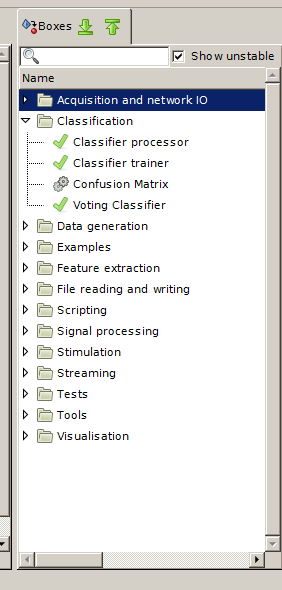
\includegraphics[height=7cm]{images/interface_bloc_ov.png}
	\caption{Interface du répertoire des blocs OpenViBE.}
	\label{fig:interface_bloc_ov_2}
\end{figure}

\subsubsection*{Description de l'espace de travail}

La partie centrale de l'interface graphique correspond à l'espace de travail d'OpenViBE. C'est ici que l'on construit les différents scénarios de l'interface cerveau-ordinateur, via des blocs fonctionnels. Chaque bloc peut être relié à un autre. On peut seulement connecter une entrée à une sortie du même type (e.g. une entrée de type "signal" vers une sortie de type "signal") (Figure : \ref{fig:interface_travail_ov_4}).

\begin{figure}[h]
	\centering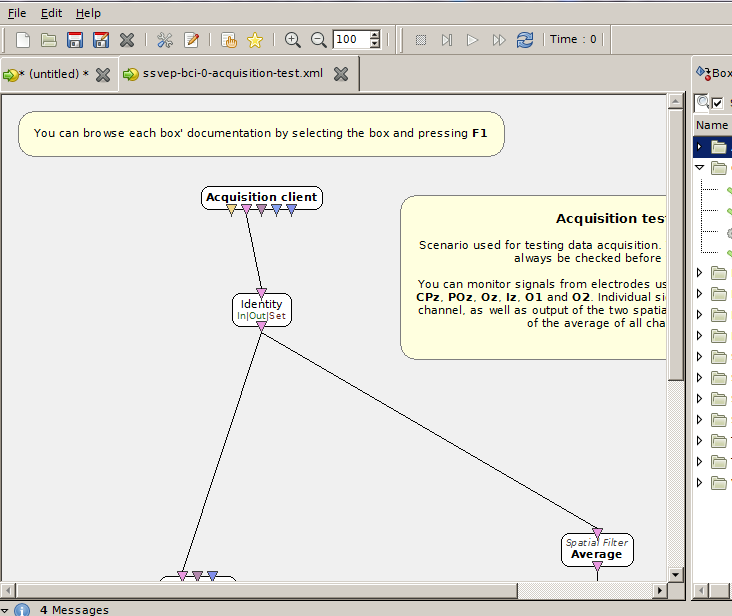
\includegraphics[height=8cm]{images/interface_travail_ov.png}
	\caption{Espace de travail d'OpenViBE.}
	\label{fig:interface_travail_ov_4}
\end{figure}


\newpage

\section*{Manipulation}

\begin{enumerate}
	\smallbreak
	\item Commencez dans un premier temps par télécharger et installer OpenViBE. Celui-ci vous servira dans la question 3. 
	\smallbreak
	\item On vous demande de coder un filtre spatial PCA sous Matlab et de traiter les données EEG contenues dans le fichier "données\_entrée.csv". Le code Matlab n'étant pas directement exécutable dans OpenViBE, vous devez utiliser la fonction Matlab "lecture\_csv.m" afin d'extraire les données EEG du fichier "données\_entrée.csv", ainsi que la fonction "ecriture\_csv.m" afin d'écrire les données après filtrage spatial vers le fichier CSV "données\_EEG\_sortie.csv".
	\smallbreak
	\item Une fois le code implémenté et vos données filtrées, on exporte les signaux vers OpenViBE. Pour cela, démarrez OpenViBE. Ouvrez ensuite le fichier "online.xml".
	\smallbreak
	\item Double-cliquez sur le bloc "CSV File Reader" et indiquez le chemin vers le fichier que vous avez généré à partir de votre code Maltab. Par défaut, ce fichier s'appelle "données\_EEG\_sortie.csv". 
	\smallbreak
	\item Double-cliquez sur le bloc "Classifier Processor" et indiquez le chemin vers le fichier "classifier.cfg" qui vous a été fourni.
	\smallbreak
	\item Double-cliquez sur le bloc "Graz motor imagery bci simulator" et indiquez le chemin vers le fichier "motor-imagery-bci-graz-stimulator.lua" qui vous a été fourni.
	\smallbreak
	\item Démarrez l'interface cerveau-ordinateur en cliquant sur le bouton "lecture". Qu'observez vous dans la fenêtre de visualisation ? 
	\smallbreak 
	\item De la même manière que dans la question 2, on vous demande à présent d'implémenter un filtre spatial ICA sous Matlab. Exportez de nouveau vos données vers OpenViBE. Qu'observez vous ? 
\end{enumerate}

